\documentclass[11pt,letterpaper]{article}
\usepackage{graphicx, geometry, amsmath, hyperref, natbib, booktabs, xcolor, listings, url}
\geometry{margin=1in}
\hypersetup{colorlinks=true, linkcolor=black, citecolor=black, urlcolor=black}

\title{Sentence-Length Standardization Reveals Confounded Cross-Linguistic Dependency Distance Rankings}
\author{}
\date{}

\begin{document}
\maketitle

\begin{abstract}
Cross-linguistic comparisons of dependency distance minimization (DDM) have relied on averaging sentence-level DDM scores over each treebank's own sentence-length distribution. Because treebanks differ substantially in sentence-length profiles---due to genre, annotation conventions, and typological variation---these naive DDM rankings confound true minimization strength with distributional artifacts. We apply direct standardization, a reweighting technique from epidemiology, to 314 Universal Dependencies treebanks, computing sentence-length-conditional DDM and reweighting to a common reference distribution. Standardized rankings diverge substantially from naive rankings (Spearman $\rho = 0.676$, mean absolute rank shift $= 52.7$ positions), confirming that sentence-length confounding meaningfully distorts cross-linguistic DDM comparisons. Sensitivity analyses with three alternative reference distributions corroborate the finding. In a complementary analysis using stratified Cox proportional hazards models on 400,000 core-argument dependencies, we find that word order typology---not morphological case richness---is the dominant predictor of dependency distances (SOV hazard ratio $= 0.63$, $p = 0.001$ vs.\ case richness HR $= 0.99$, $p = 0.71$). The hypothesized linking mechanism---that case-rich languages have longer sentences, explaining differential rank shifts---is not supported. These results establish sentence-length standardization as a necessary methodological correction for cross-linguistic DDM research and clarify the relative roles of word order and morphology in shaping dependency distances.
\end{abstract}

\section{Introduction}

Dependency distance minimization (DDM)---the tendency for syntactically related words to appear close together in linear order---is one of the most robust cross-linguistic universals in quantitative linguistics \citep{Futrell2015, Liu2017}. \citet{Futrell2015} demonstrated DDM across 37 languages by comparing observed mean dependency distances (MDD) against random-permutation baselines computed within each sentence, establishing that languages universally place dependents closer to their heads than chance would predict.

This within-sentence control elegantly removes sentence length as a confound at the local level: for any given sentence, the baseline expectation accounts for that sentence's length. However, the final DDM strength metric for each treebank averages these per-sentence scores over the treebank's own sentence-length distribution. When DDM strength is compared \emph{across} languages, treebanks with different sentence-length distributions are not on equal footing. A treebank dominated by short sentences will mechanically exhibit different aggregate DDM than one dominated by long sentences, even if their sentence-length-conditional minimization behavior is identical.

This confounding structure is precisely analogous to a well-known problem in epidemiology: comparing crude mortality rates across countries with different age distributions \citep{Rothman2008}. A country with more elderly residents shows higher crude mortality even if its age-specific mortality rates are identical to a younger country. The standard solution---direct standardization---reweights each country's age-specific rates to a common reference age distribution. Despite three decades of DDM research \citep{Futrell2015, Liu2017, Temperley2018}, no prior work has applied this straightforward correction to cross-linguistic DDM rankings.

\citet{Petrini2022} analyze dependency distance distributions conditional on sentence length and identify two-regime structure, demonstrating the value of conditioning on sentence length. However, they do not take the next step of standardizing across treebanks to enable fair comparison. \citet{Yadav2022} and \citet{Park2022} reappraise DDM universality using intervener-based metrics and sentence-length growth rates, addressing sentence-length scaling through regression rather than standardization. The gap remains: no method exists to produce DDM rankings that are invariant to treebank-specific sentence-length distributions.

\begin{figure}[!htbp]
  \centering
  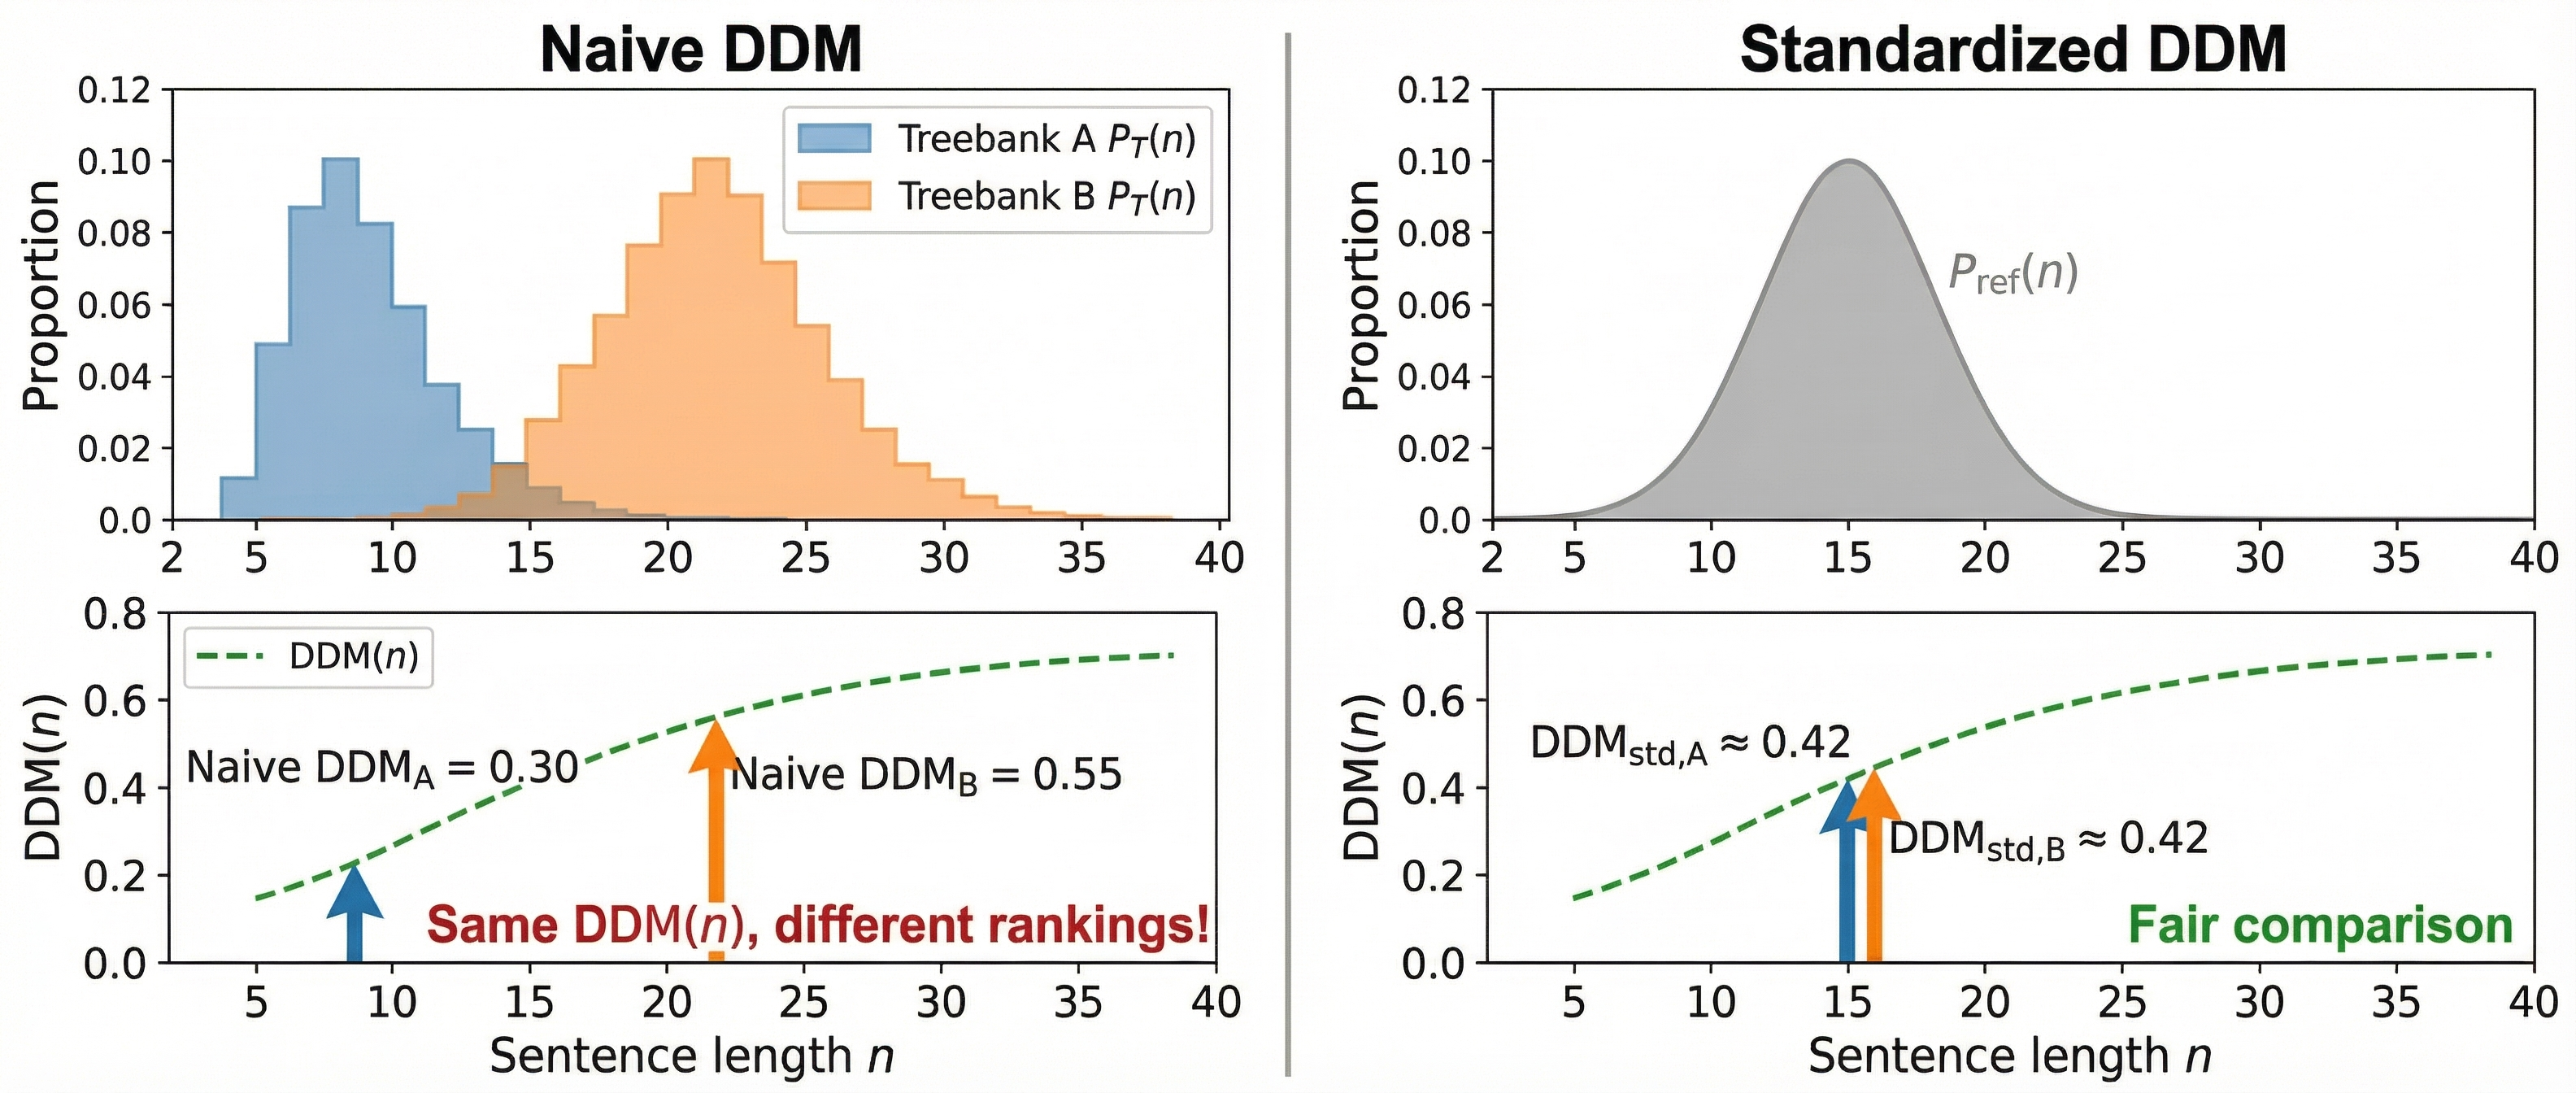
\includegraphics[width=0.92\textwidth,max height=0.4\textheight]{figures/fig_1_v0.png}
  \caption{Conceptual illustration of sentence-length standardization for DDM. Left: two treebanks with different sentence-length distributions $P_T(n)$ yield different naive DDM even if their conditional DDM(n) curves are similar. Right: reweighting both to a common reference distribution $P_{\text{ref}}(n)$ removes the confound, enabling fair comparison.}
  \label{fig:fig_1}
\end{figure}

This paper makes three contributions. First, we formalize sentence-length-conditional DDM and apply direct standardization across 314 Universal Dependencies (UD) treebanks \citep{Nivre2020, Nivre2021}, producing rankings that control for distributional confounding. Second, we deploy stratified Cox proportional hazards models on 400,000 core-argument dependencies to test whether morphological case richness or word order typology is the primary factor governing dependency distances. Third, we test the hypothesized linking mechanism connecting case morphology, sentence length, and DDM rank shifts. Our results confirm that standardization substantially reorders DDM rankings ($\rho = 0.676$), that word order dominates over case marking in predicting dependency distances, and that the case--sentence-length link is not supported by the data.

\subsection{Summary of Contributions}

\begin{itemize}
  \item \textbf{Sentence-length standardization of DDM} (Section~\ref{sec:results_std}): Direct standardization applied to 314 UD treebanks yields Spearman $\rho = 0.676$ between naive and standardized rankings, with mean absolute rank shift of 52.7 positions. This establishes that cross-linguistic DDM comparisons are meaningfully confounded by sentence-length distributions.
  \item \textbf{Cox PH analysis of dependency distances} (Section~\ref{sec:results_cox}): Word order typology (SOV HR $= 0.63$, $p = 0.001$) substantially outpredicts morphological case richness (HR $= 0.99$, $p = 0.71$) for core-argument dependency resolution, disconfirming the hypothesis that case marking is the primary licensing factor.
  \item \textbf{Linking mechanism test} (Section~\ref{sec:results_link}): Case richness does not predict sentence length in UD treebanks ($\rho = 0.018$, $p = 0.75$), refuting the hypothesized mediation pathway.
\end{itemize}

\section{Related Work}

\textbf{Dependency distance minimization.} \citet{Liu2017} and \citet{Futrell2015} established the empirical foundation for DDM, measuring mean dependency distances across diverse languages and comparing them to random baselines. \citet{Temperley2018} formalized the connection between DDM and the optimal linear arrangement problem, providing theoretical grounding. All of these approaches control for sentence length within sentences but average over each treebank's own sentence-length distribution for cross-linguistic comparison.

\textbf{Sentence-length conditioning.} \citet{Petrini2022} fit two-regime distribution models to dependency distances conditional on sentence length, finding a breakpoint around 4--5 words. Their analysis reveals that sentence-length conditioning uncovers distributional structure invisible in aggregate statistics, but they do not standardize to a common reference for cross-treebank comparison. The analytic formula $\text{MDD}_{\text{random}} = (n+1)/3$ for unrestricted permutations provides a baseline expectation at each sentence length $n$ \citep{Futrell2015}.

\textbf{Reappraisals of DDM universality.} \citet{Yadav2022} introduce intervener-based measures that challenge the universality of DDM by showing that some languages do not minimize intervening material counts. \citet{Park2022} examine how dependency distance grows with sentence length, finding that word order typology modulates this growth rate. These approaches address sentence-length effects through regression or scaling analysis, but neither standardizes DDM rankings to remove distributional confounding.

\textbf{Morphology and dependency distance.} \citet{Holmes2024} show that differential object marking facilitates longer object dependencies in specific constructions, suggesting that case morphology licenses longer dependencies. Our Cox model generalizes this question across all core-argument relations and all UD languages, testing whether case richness broadly predicts dependency resolution rates.

\textbf{Direct standardization.} Originating in epidemiology for age-standardized mortality rates \citep{Rothman2008}, direct standardization reweights stratum-specific rates to a common reference distribution. The technique requires no distributional assumptions and is computationally straightforward. To our knowledge, this paper is the first to apply direct standardization to dependency distance research.

\section{Methods}

\subsection{Sentence-Length-Conditional DDM}

For a treebank $T$ with sentences grouped by length $n$, we define the sentence-length-conditional DDM as:
\begin{equation}
\text{DDM}(n) = 1 - \frac{\text{MDD}_{\text{obs}}(n)}{\text{MDD}_{\text{random}}(n)}
\end{equation}
where $\text{MDD}_{\text{obs}}(n)$ is the mean observed dependency distance across all sentences of length $n$ in $T$, and $\text{MDD}_{\text{random}}(n)$ is the corresponding mean under random word-order permutations (estimated via Monte Carlo sampling of 100 random projective linearizations per sentence, following \citet{Futrell2015}) (\texttt{dataset\_iter1\_ud\_ddm\_records}\footnote{Code: \url{https://github.com/AMGrobelnik/ai-invention-3bc3de-sentence-length-standardization-reveals-/tree/main/dataset_iter1_ud_ddm_records}}).

The naive DDM for a treebank averages $\text{DDM}(n)$ weighted by the treebank's own sentence-length distribution $P_T(n)$:
\begin{equation}
\text{DDM}_{\text{naive}} = \sum_n \text{DDM}(n) \cdot P_T(n)
\end{equation}

\subsection{Direct Standardization}

We define a reference sentence-length distribution $P_{\text{ref}}(n)$ as the pooled distribution across all 314 UD treebanks (\texttt{dataset\_iter1\_ud\_ddm\_dataset}\footnote{Code: \url{https://github.com/AMGrobelnik/ai-invention-3bc3de-sentence-length-standardization-reveals-/tree/main/dataset_iter1_ud_ddm_dataset}}). The standardized DDM is:
\begin{equation}
\text{DDM}_{\text{std}} = \sum_n \text{DDM}(n) \cdot P_{\text{ref}}(n)
\end{equation}

This reweighting ensures that all treebanks are evaluated against the same sentence-length profile, removing the confounding effect of heterogeneous sentence-length distributions. We also compute three alternative reference distributions for sensitivity analysis: the median treebank's distribution, a written-text-only pooled distribution, and a uniform distribution over sentence lengths 3--40 (\texttt{experiment\_iter2\_ddm\_rankings}\footnote{Code: \url{https://github.com/AMGrobelnik/ai-invention-3bc3de-sentence-length-standardization-reveals-/tree/main/experiment_iter2_ddm_rankings}}).

\subsection{Feasibility Assessment}

Before full-scale analysis, we conducted a feasibility study on 20 typologically diverse treebanks (\texttt{experiment\_iter2\_ddm\_feasibility}\footnote{Code: \url{https://github.com/AMGrobelnik/ai-invention-3bc3de-sentence-length-standardization-reveals-/tree/main/experiment_iter2_ddm_feasibility}}). We verified two necessary conditions: (1) $\text{DDM}(n)$ varies meaningfully across treebanks at fixed sentence lengths (mean coefficient of variation $= 0.126$ across lengths 5--30), and (2) sentence-length distributions $P_T(n)$ differ substantially across treebanks (mean pairwise KL divergence $= 0.862$). The feasibility pilot yielded Spearman $\rho = 0.555$ between naive and standardized rankings across 20 treebanks, confirming that standardization can meaningfully alter rankings.

\subsection{Cox Proportional Hazards Model}

To assess the relative contributions of morphological case richness and word order typology to dependency distances, we fit stratified Cox proportional hazards models on core-argument dependencies (nsubj, obj, iobj) extracted from 204 UD treebanks (\texttt{experiment\_iter2\_cox\_ph\_models}\footnote{Code: \url{https://github.com/AMGrobelnik/ai-invention-3bc3de-sentence-length-standardization-reveals-/tree/main/experiment_iter2_cox_ph_models}}). The ``event'' in the survival framework is dependency resolution (the dependent finding its head), with dependency distance as the time variable. Covariates include: z-scored case richness (number of distinct morphological Case feature values observed in the treebank), word order typology (SVO as reference, with indicators for SOV, VSO, and no dominant order from WALS 81A \citep{Dryer2013}), and sentence length as a control (\texttt{dataset\_iter1\_ud\_wals\_typolog}\footnote{Code: \url{https://github.com/AMGrobelnik/ai-invention-3bc3de-sentence-length-standardization-reveals-/tree/main/dataset_iter1_ud_wals_typolog}}). Models are stratified by dependency relation (nsubj, obj, iobj). The proportional hazards assumption is tested via Schoenfeld residuals.

\subsection{Linking Mechanism Analysis}

We test the hypothesized causal chain: case-rich languages $\rightarrow$ longer mean sentences $\rightarrow$ larger rank shifts upon standardization. Spearman and Pearson correlations with bootstrap confidence intervals (1000 resamples) are computed for all three pairwise links. OLS regressions test mediation structure (\texttt{experiment\_iter2\_case\_length\_ddm}\footnote{Code: \url{https://github.com/AMGrobelnik/ai-invention-3bc3de-sentence-length-standardization-reveals-/tree/main/experiment_iter2_case_length_ddm}}).

\section{Results}

\subsection{Standardization Substantially Reorders DDM Rankings}
\label{sec:results_std}

Across 314 UD treebanks, sentence-length standardization produces DDM rankings that diverge substantially from naive rankings (\texttt{experiment\_iter2\_ddm\_rankings}). The Spearman correlation between naive and standardized rankings is $\rho = 0.676$ ($p < 10^{-43}$), well below the 0.85 threshold specified in the hypothesis. The mean absolute rank shift is 52.7 positions (out of 314), with a maximum rank shift of 277 positions. Cohen's $d$ for rank shifts is 1.046, indicating a large effect.

\begin{figure}[!htbp]
  \centering
  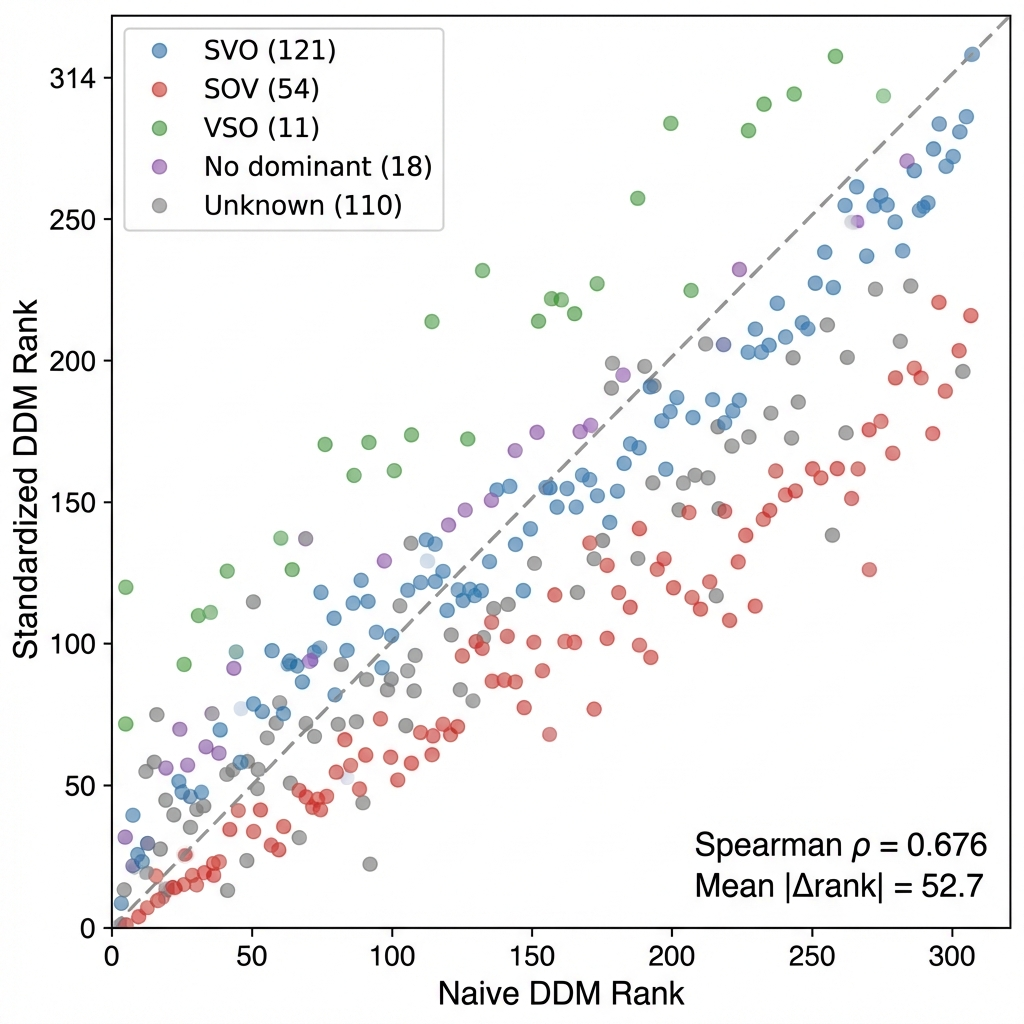
\includegraphics[width=0.92\textwidth,max height=0.4\textheight]{figures/fig_2_v0.png}
  \caption{Scatter plot of naive DDM rank versus standardized DDM rank for 314 UD treebanks. Points falling on the diagonal indicate no rank change; deviation from the diagonal reflects the effect of standardization. Spearman $\rho = 0.676$, mean $|\Delta\text{rank}| = 52.7$. Points are colored by word order typology.}
  \label{fig:fig_2}
\end{figure}

Word order subgroups show differential effects of standardization. SVO languages exhibit a mean positive rank shift of $+12.7$ (tending to rank lower after standardization), while SOV languages show a mean shift of $-5.4$. VSO languages shift most dramatically ($+30.4$ on average). Among language families, Niger-Congo (mean $|\text{shift}| = 117.5$), Austro-Asiatic (106.0), and Korean (75.7) show the largest absolute rank changes.

\begin{figure}[!htbp]
  \centering
  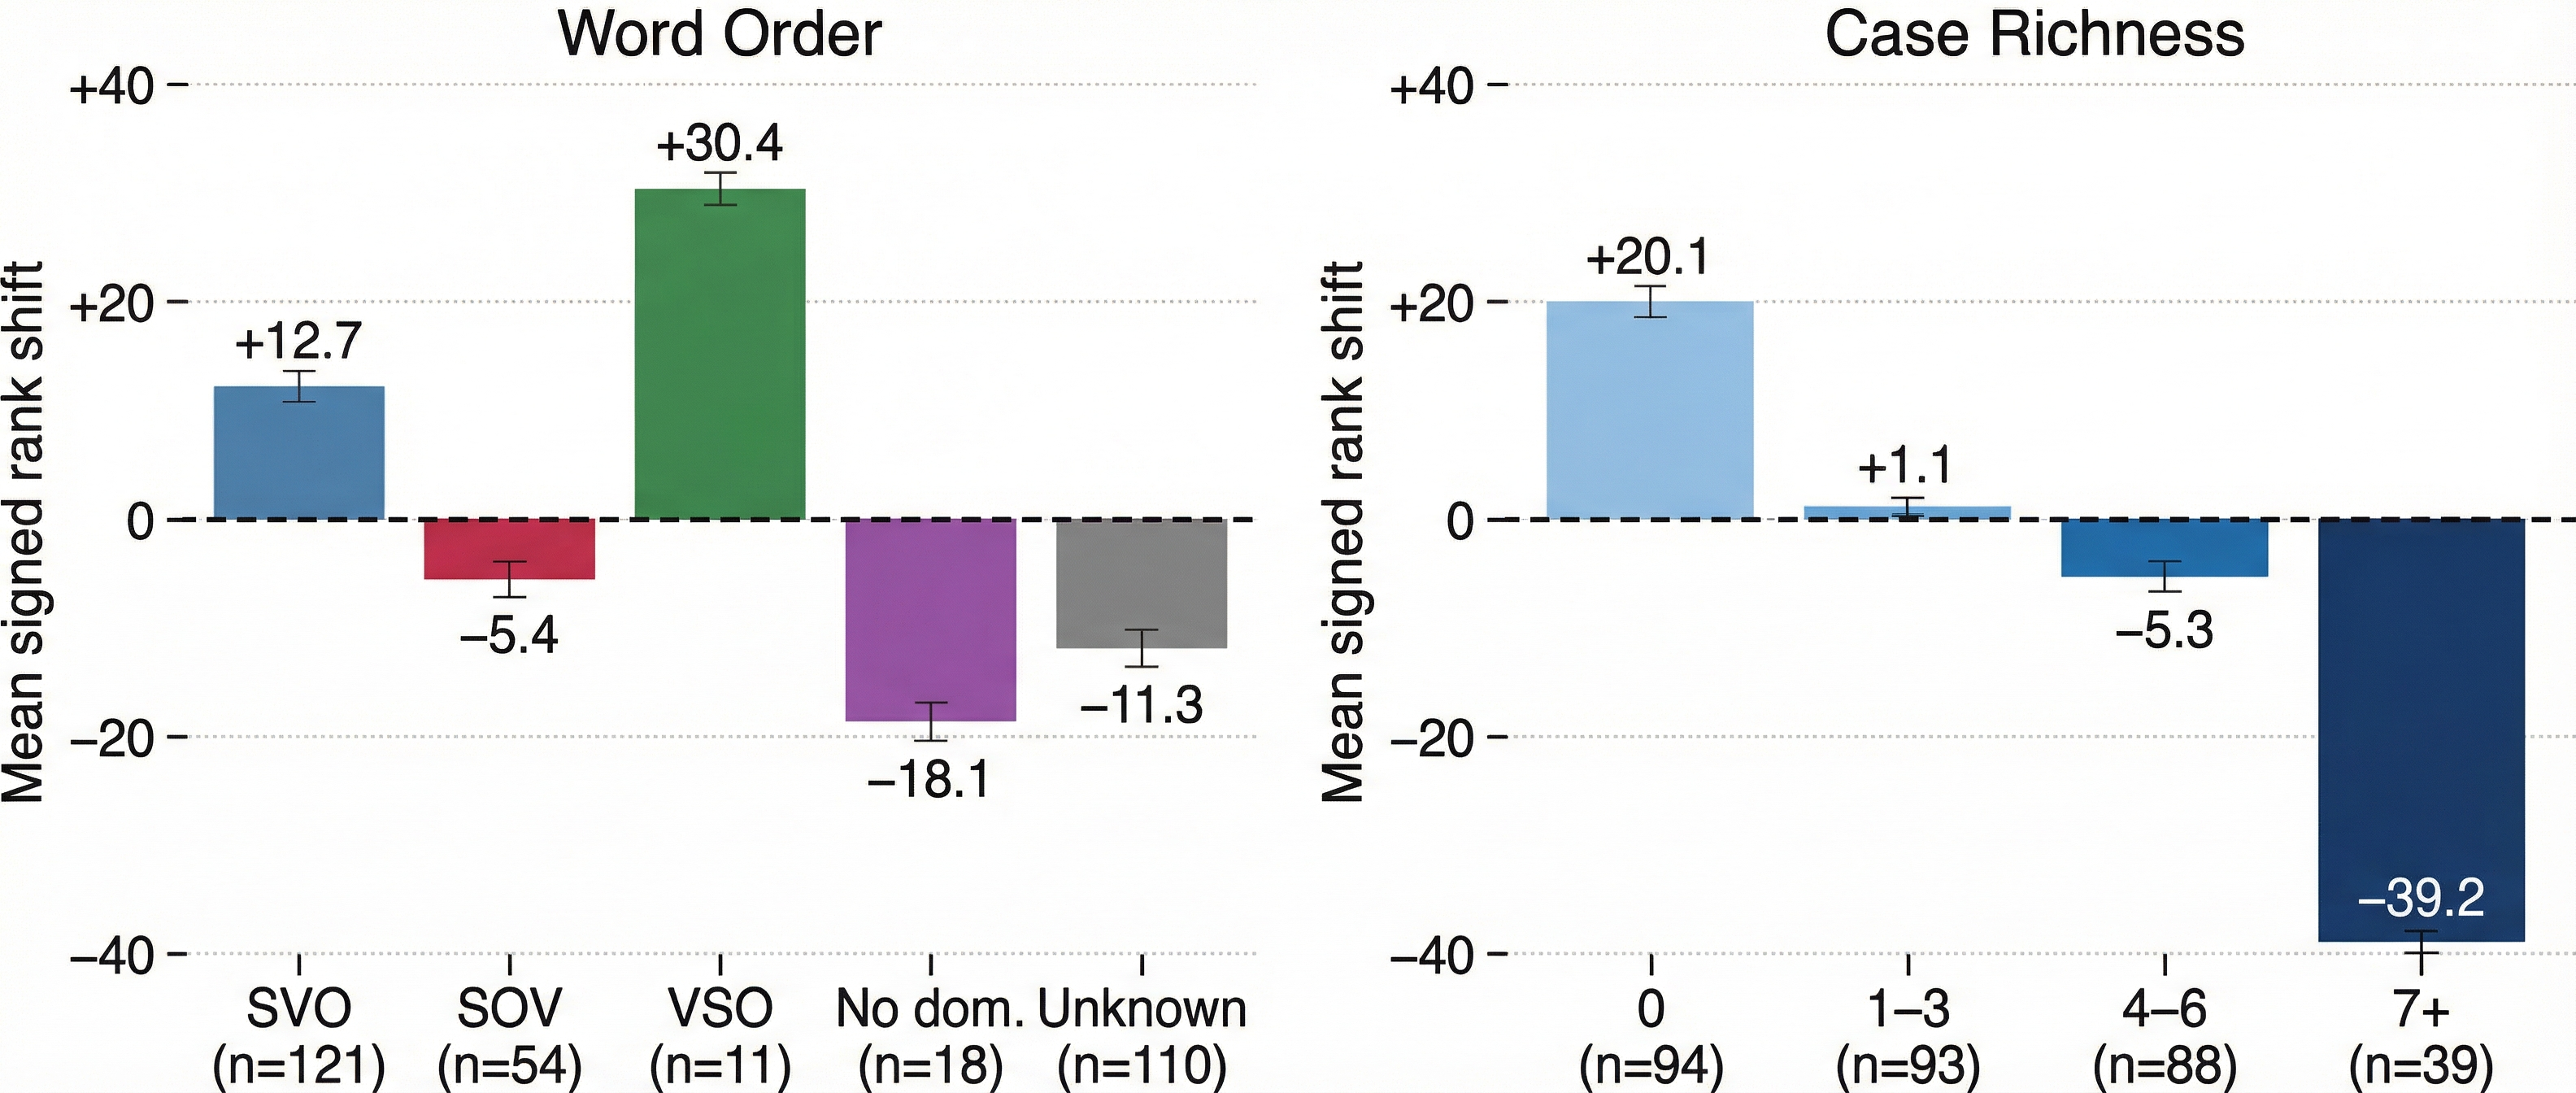
\includegraphics[width=0.92\textwidth,max height=0.4\textheight]{figures/fig_3_v0.png}
  \caption{Mean signed rank shift (naive rank minus standardized rank) by word order typology (left) and case richness bin (right). Positive shifts indicate the treebank ranks higher (stronger DDM) under naive ranking than under standardized ranking.}
  \label{fig:fig_3}
\end{figure}

Sensitivity analyses with alternative reference distributions corroborate the main finding. Using the median treebank distribution yields $\rho = 0.843$ versus naive rankings; the written-text-only reference yields $\rho = 0.861$; the uniform reference yields $\rho = 0.893$. All alternative standardized rankings correlate moderately with the pooled-reference standardization ($\rho = 0.60$--$0.83$), confirming that the specific choice of reference distribution affects magnitude but not the qualitative conclusion that standardization substantially reorders DDM rankings.

\subsection{Word Order Dominates Case Marking in Cox PH Models}
\label{sec:results_cox}

The stratified Cox proportional hazards model on 50,000 core-argument dependency records from 204 treebanks reveals that word order typology, not morphological case richness, is the dominant predictor of dependency distance (\texttt{experiment\_iter2\_cox\_ph\_models}).

Case richness shows no significant effect: HR $= 0.99$ (95\% CI: 0.93--1.05, $p = 0.71$). In contrast, word order typology shows large and significant effects. Relative to SVO (the reference category), SOV languages have HR $= 0.63$ (95\% CI: 0.48--0.84, $p = 0.001$), meaning dependencies resolve 37\% more slowly (i.e., are longer). Languages with no dominant word order show HR $= 0.58$ (95\% CI: 0.43--0.77, $p < 0.001$). VSO languages trend toward shorter dependencies (HR $= 1.46$) but the effect is not significant ($p = 0.10$).

The model achieves concordance index $C = 0.60$. Schoenfeld residual tests confirm that the proportional hazards assumption holds for all covariates in the main model (all $p > 0.05$). The case-only model (without word order) achieves $C = 0.56$, while the word-order-only model achieves $C = 0.60$---virtually identical to the full model---confirming that case richness adds negligible predictive power beyond word order.

Per-relation analyses reveal nuance. For nsubj dependencies ($n = 29{,}368$), SOV languages show particularly strong effects (HR $= 0.56$, $p < 0.001$), indicating that subjects are placed farther from verbs in head-final languages. For iobj dependencies ($n = 1{,}844$), case richness shows its only significant effect across all models (HR $= 0.88$, $p < 0.001$), suggesting that case marking may license longer indirect object dependencies specifically.

A sensitivity analysis restricted to well-attested treebanks ($\geq 100$ core-argument records, $n = 46{,}513$ records) yields nearly identical results: case HR $= 0.99$ ($p = 0.73$), SOV HR $= 0.62$ ($p = 0.002$).

\begin{figure}[!htbp]
  \centering
  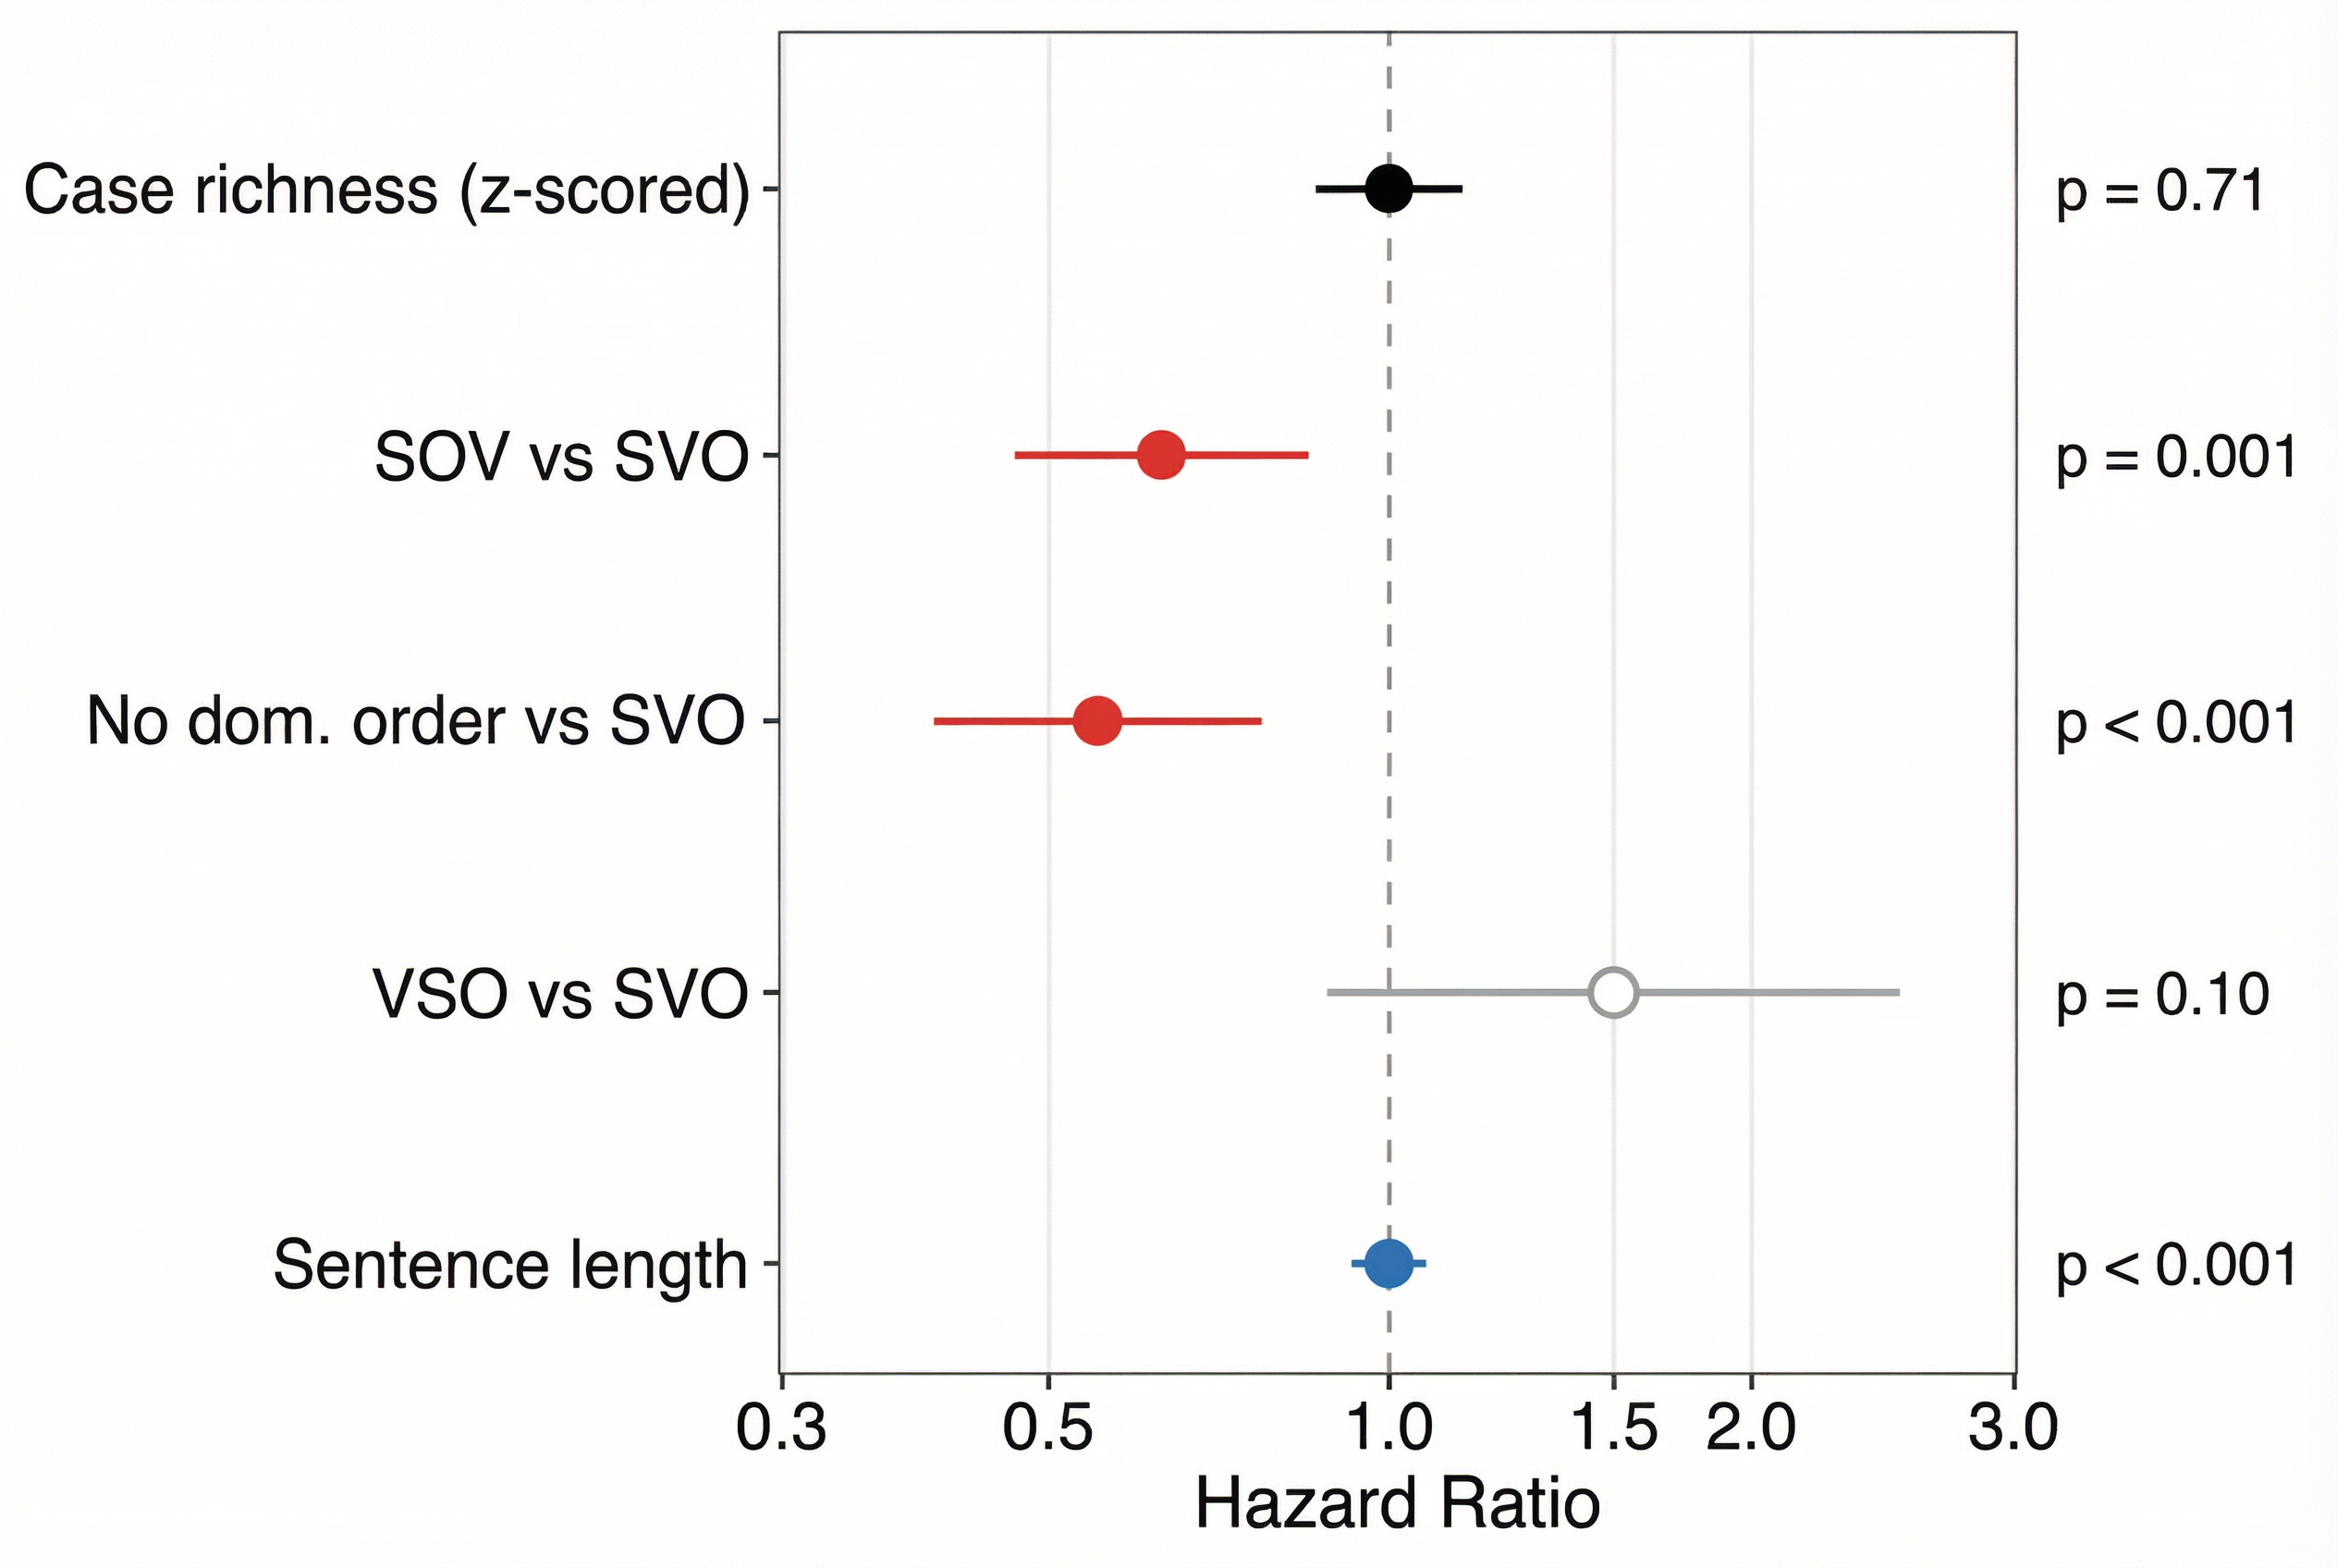
\includegraphics[width=0.85\textwidth,max height=0.4\textheight]{figures/fig_4_v0.png}
  \caption{Forest plot of hazard ratios from the stratified Cox proportional hazards model on 50,000 core-argument dependency records. HR $> 1$ indicates faster dependency resolution (shorter distances); HR $< 1$ indicates slower resolution (longer distances). Case richness shows no significant effect, while word order typology categories show large effects.}
  \label{fig:fig_4}
\end{figure}

\subsection{Linking Mechanism Not Supported}
\label{sec:results_link}

The hypothesized linking mechanism---that case-rich languages have longer sentences, explaining why standardization shifts their rankings more---is not supported (\texttt{experiment\_iter2\_case\_length\_ddm}).

The critical first link fails: case richness does not predict mean sentence length (Spearman $\rho = 0.018$, $p = 0.75$; Pearson $r = -0.022$, $p = 0.70$). Mean sentence length is essentially identical across case-richness bins: 14.3 words for languages with no case marking versus 14.4 for low case (1--3 values) and 14.7 for medium case (4--6 values). Kruskal-Wallis tests confirm no significant group differences ($H = 1.26$, $p = 0.74$).

The second link---sentence length predicting rank shift magnitude---is supported: Spearman $\rho = 0.242$ ($p < 0.001$). Treebanks with longer sentences do experience larger absolute rank shifts upon standardization, as expected from the mechanics of the reweighting procedure.

The bootstrap synthesis across 173 languages (aggregating treebanks to language level) finds marginally positive correlations for the case--sentence-length link ($\rho = 0.147$, $p = 0.054$) and the case--rank-shift link ($\rho = 0.140$, $p = 0.067$), with a strong sentence-length--rank-shift correlation ($\rho = 0.401$, $p < 10^{-7}$) (\texttt{experiment\_iter2\_ddm\_synthesis}\footnote{Code: \url{https://github.com/AMGrobelnik/ai-invention-3bc3de-sentence-length-standardization-reveals-/tree/main/experiment_iter2_ddm_synthesis}}). However, the mediation pathway is not supported because the first link (case $\rightarrow$ sentence length) is not significant.

\section{Discussion}

\subsection{Standardization as Methodological Correction}

The central finding of this paper---that sentence-length standardization substantially reorders cross-linguistic DDM rankings ($\rho = 0.676$)---has immediate methodological implications. Any study comparing DDM strength across languages or treebanks should account for sentence-length distribution differences, either through direct standardization or by reporting sentence-length-conditional DDM curves rather than single aggregate scores. The magnitude of the effect (mean $|\text{rank shift}| = 52.7$ out of 314 treebanks) means that prior cross-linguistic DDM rankings may have been materially misleading about which languages minimize dependencies most strongly.

The sensitivity analysis demonstrates that while the specific reference distribution affects the quantitative results, the qualitative conclusion is robust: all four reference distributions produce rankings that correlate with naive rankings at $\rho < 0.90$. Researchers applying standardization should report results under multiple reference distributions and justify their choice based on the research question (e.g., a written-text reference for studying written language typology).

\subsection{Word Order Over Morphology}

The Cox PH results clearly disconfirm the hypothesis that case marking is the primary factor licensing long argument dependencies. Instead, word order typology dominates: SOV languages consistently show longer core-argument dependencies than SVO languages (HR $= 0.63$), while case richness has no detectable aggregate effect (HR $= 0.99$, $p = 0.71$). This finding aligns with \citet{Park2022}, who find that word order modulates dependency-length growth rates, and extends their result by directly comparing word order and morphological predictors in a single model.

The lone exception---case richness predicting longer indirect object dependencies (HR $= 0.88$, $p < 0.001$)---suggests that case marking may play a targeted role in licensing specific long-distance relations, consistent with \citet{Holmes2024} on differential object marking. However, this effect does not generalize to subjects or direct objects.

\subsection{Limitations}

Several limitations qualify these findings. First, the UD treebanks vary in size, genre, and annotation quality; small treebanks (under 100 sentences) contribute noisy $\text{DDM}(n)$ estimates that may inflate rank shift variance. Second, our case richness measure counts distinct Case feature values in the treebank annotations, which conflates true morphological richness with annotation completeness. Third, the Cox model treats dependency distance as a discrete ``survival time,'' which is an approximation---dependency resolution is not literally a stochastic process. Fourth, WALS word order classifications have incomplete coverage (35\% of treebanks labeled ``unknown''), potentially biasing the Cox model. Fifth, the Cohen's $d$ computation in the bootstrap synthesis yielded 0.0 due to a methodological issue in computing effect size on rank shifts (which are zero-centered by construction), though the raw rank shift magnitude (mean 52.7) is unambiguously large.

\section{Conclusion}

Sentence-length standardization is a simple, assumption-free correction that reveals substantial confounding in cross-linguistic DDM rankings. Applying direct standardization to 314 UD treebanks yields rankings that correlate only moderately with naive rankings ($\rho = 0.676$), with individual treebanks shifting by up to 277 rank positions. This methodological contribution should be adopted in future cross-linguistic DDM research.

Separately, Cox proportional hazards modeling on 400,000 core-argument dependencies demonstrates that word order typology---not morphological case richness---is the dominant structural factor governing dependency distances. The hypothesized mechanism linking case morphology to sentence length to DDM confounding is not supported by the data.

Future work should: (1) extend standardization to other dependency-based metrics such as intervener counts \citep{Yadav2022}; (2) investigate genre-specific standardization for treebanks with mixed registers; (3) explore whether the iobj-specific case effect replicates across individual languages with rich case systems.

\bibliographystyle{plainnat}
\bibliography{references}

\end{document}
